\newpage
\section{Auswertung}
\label{sec:Auswertung}
%%%%Tabelle: Gerätedaten
\begin{table}
	\centering
	\begin{tabular}{c c}
	\toprule
	\multicolumn{2}{c}{Daten von Gerät 1} \\
	%{Bauteil} & {Daten} \\
	\midrule
 Induktivität L & 294.45 \\
 Kapazität C    & 294.45 \\
 Widerstand $R_1$ & 294.35 \\
 Widerstand $R_2$ & 293.45 \\
	\bottomrule
	\end{tabular}
	\caption{Daten der in Gerät 1 verwendeten Bauteile.}
	\label{tab:geraet}
\end{table}
%%%%%%%%%Schwingfall Plot
\begin{figure}[h]
		\centering
		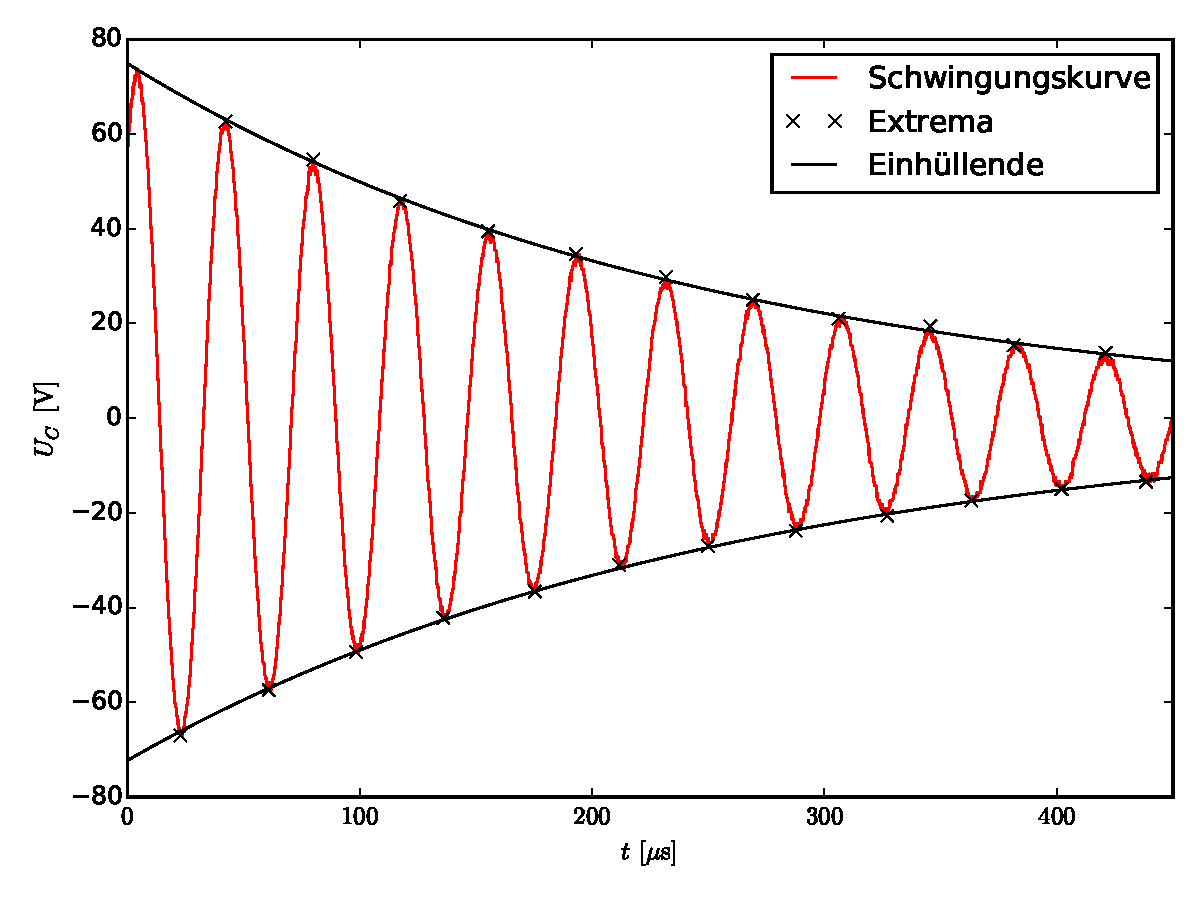
\includegraphics[width=\textwidth]{build/plot_schwingungskurve.pdf}
		\caption{Verhalten der Spannung für den Schwingfall.}
\end{figure}

%%%%%%%Schwingfall, logarithmischer Plot
\begin{figure}[h]
		\centering
		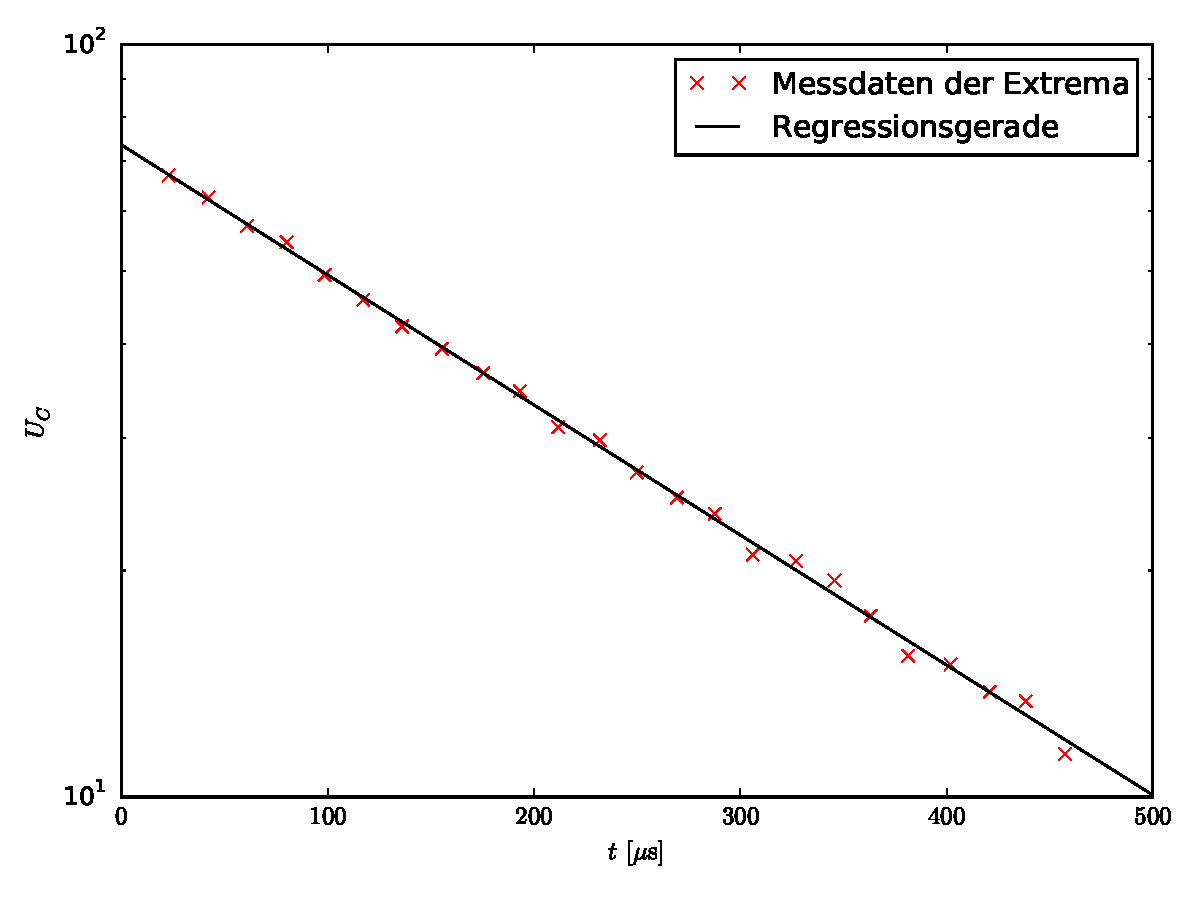
\includegraphics[width=\textwidth]{build/plot_einhuellende_semilog.pdf}
		\caption{Einhüllende der Schwingungskurve, aufgetragen auf halblogarithmischer Skala.}
\end{figure}
%%%%%%%%Tabelle: Extremwerte der Spannung
\begin{table}
	\centering
	\begin{tabular}{S[table-format=3.0] S[table-format=2.2] S[table-format=3.0] S[table-format=2.2]}
	\toprule
	{$t\:/{\si{\micro\second}}$} & {$U_\mathup{C,min}\:/{\si{\volt}}$} &{$t\:/{\si{\micro\second}}$}& {$U_\mathup{C,max}\:/{\si{\volt}}$} \\
	\midrule
 42 & 62.60 &  23 & -67.00\\
 80 & 54.60 &  61 & -57.40\\
117 & 45.80 &  98 & -49.40\\
155 & 39.40 & 136 & -42.20\\
193 & 34.60 & 175 & -36.60\\
232 & 29.80 & 212 & -31.00\\
269 & 25.00 & 250 & -27.00\\
306 & 21.00 & 288 & -23.80\\
346 & 19.40 & 327 & -20.60\\
381 & 15.40 & 363 & -17.40\\
421 & 13.80 & 402 & -15.00\\
457 & 11.40 & 438 & -13.40\\
	\bottomrule
	\end{tabular}
	\caption{Extrema der Spannungswerte.}
	\label{tab:extrema}
\end{table}

\subsection{Aperiodischer Grenzfall im gedämpften Schwingkreis}
%%%%%%%%%%%%%%%%%Aperiodischer Grenzfall, Screenshot
\begin{figure}[h]
		\centering
		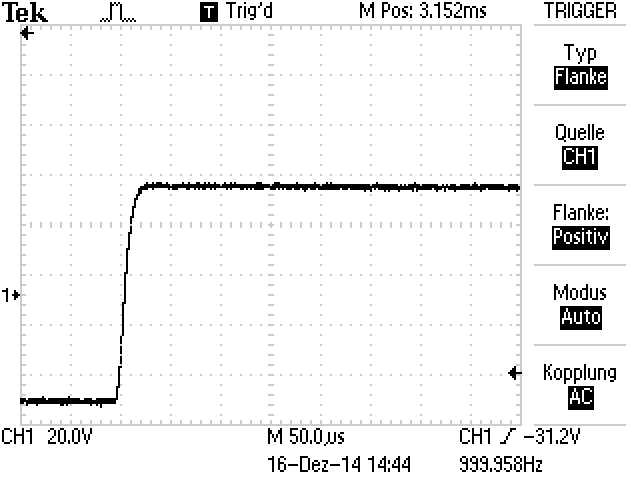
\includegraphics[width=0.5\textwidth]{Bilder/Aperiodischer.JPG}
		\caption{Screenshot des aperiodischen Grenzfalls.}
\end{figure}

%%%%%%%%%%%%%%%%%Schwingfall, Screenshot
\begin{figure}[h]
		\centering
		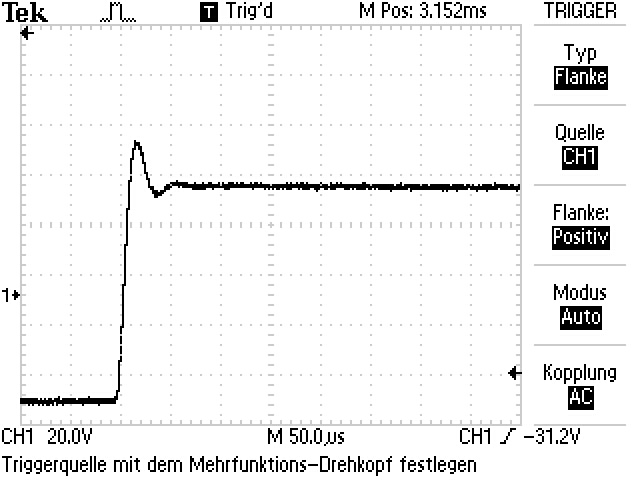
\includegraphics[width=0.5\textwidth]{Bilder/Schwingfall.JPG}
		\caption{Screenshot des Schwingfalls.}
\end{figure}
%%%%%%%%%%%%%%%%%kriechfall, Screenshot
\begin{figure}[h]
		\centering
		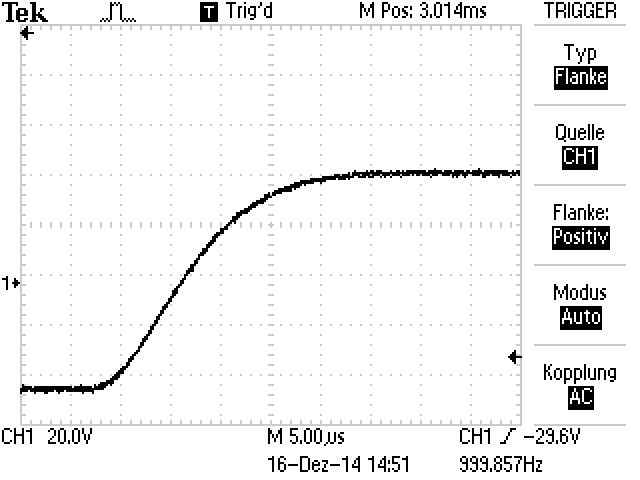
\includegraphics[width=0.5\textwidth]{Bilder/Kriechfall1.JPG}
		\caption{Screenshot des Kriechfalls.}
\end{figure}

\subsection{Frequenzabhängigkeit der Kondensatorspannung}
%%%%%tabelle: kondensatorspannung,, frequenzabh.
\begin{table}
	\centering
\setlength{\tabcolsep}{2mm}
\begin{tabular}{cc}
	\begin{tabular}{S[table-format=2.1] S[table-format=3.0] S[table-format=2.1] }
	\toprule
	{$f\:/{\si{\kilo\hertz}}$} & {$U_\mathup{C}\:/{\si{\volt}}$} & {$U_\mathup{0}\:/{\si{\volt}}$} \\
	\midrule

10.0 &  48 & 44.0\\
11.0 &  52 & 44.0\\
12.0 &  54 & 44.0\\
13.0 &  58 & 44.0\\
14.0 &  60 & 44.0\\
15.0 &  64 & 44.0\\
16.0 &  66 & 44.0\\
17.0 &  72 & 44.0\\
18.0 &  78 & 44.0\\
19.0 &  84 & 44.0\\
20.0 &  92 & 43.2\\
20.5 &  96 & 43.2\\
21.0 & 102 & 43.2\\
21.5 & 108 & 43.2\\
22.0 & 114 & 43.2\\
22.5 & 120 & 42.4\\
23.0 & 128 & 42.4\\
23.5 & 136 & 42.4\\
24.0 & 142 & 42.4\\
24.5 & 150 & 42.4\\
25.0 & 156 & 41.6\\
25.5 & 158 & 41.6\\
26.0 & 160 & 41.6\\
26.5 & 158 & 40.8\\
27.0 & 152 & 40.8\\
27.5 & 144 & 40.8\\
\bottomrule
	\end{tabular}
&	
	\begin{tabular}{S[table-format=2.1] S[table-format=3.0] S[table-format=2.1] }
	\toprule
	{$f\:/{\si{\kilo\hertz}}$} & {$U_\mathup{C}\:/{\si{\volt}}$} & {$U_\mathup{0}\:/{\si{\volt}}$} \\
	\midrule
28.0 &  136.0   & 40.8\\
28.5 &  128.0 	& 41.6\\
29.0 &  118.0 	& 41.6\\
29.5 &  108.0 	& 41.6\\
30.0 &  100.0 	& 41.6\\
30.5 &   94.0 	& 41.6\\
31.0 &   88.0 	& 42.4\\
32.0 &   76.0 	& 43.2\\
33.0 &   66.0 	& 43.2\\
34.0 &   56.0 	& 43.2\\
35.0 &	 49.0	& 43.2\\
36.0 &	 44.8 	& 43.2\\
37.0 &	 40.8 	& 43.2\\
38.0 &	 36.8 	& 43.2\\
39.0 &	 33.6 	& 43.2\\
40.0 &	 30.8 	& 43.2\\
41.0 &	 28.4 	& 43.2\\
42.0 &	 26.4 	& 43.2\\
43.0 &	 24.4 	& 43.2\\
44.0 &	 22.8 	& 43.2\\
45.0 &	 21.6 	& 43.2\\
46.0 &	 20.0 	& 43.2\\
47.0 &	 18.8 	& 43.2\\
48.0 &	 18.0 	& 43.2\\
49.0 &	 16.8 	& 43.2\\
50.0 &	 16.0 	& 43.2\\
\bottomrule
\end{tabular}
\end{tabular}
	\caption{Messdaten der Kondensator- und Generatorspannung zu verschiedenen Frequenzen.}
	\label{tab:f_U}
\end{table}
\subsection{frequenzabhängigkeit der Phasendifferenz}
